\section[EASY Suite工具]{EASY Suite工具\\The EASY Suites}
本章和接下来的章节包含特别的教育工具。这些常见的例子你可以在大多数教科书上找到,例子中大多数的计算描述在相关的MATLAB文件中。我们将其命名为easy1$\sim$easy18的M文件。它们发布为两个部分:第一部分easy1$\sim$easy10是Borre在2003提供的。第二部分easy11$\sim$easy18发布在“Inside GNSS”期刊上。(Borre(2009a)、Borre(2009b)、Borre(2009c)、Borre (2010a)、Borre(2010b)、Borre(2010c)) 

这些文件的原始观测数据正在被维护。这个决定意味着这些文件在本书中看起来是没有归类的。为了补救这种情况我们在下一页提供了这些文件的一个表格\ref{tab:9.1}。

EASY Suite工具从2000年创建用于帮助其他人理解如何使用MATLAB 代码实现GPS定位。我们为第一部分的基础性的文件构建了一个新的专题。这个专题中包含那些能让其他人能够顺利理解的复杂代码。第二部分是其他人请求能够提供的更有价值的专业代码。
\begin{figure}[H]
	\centering
	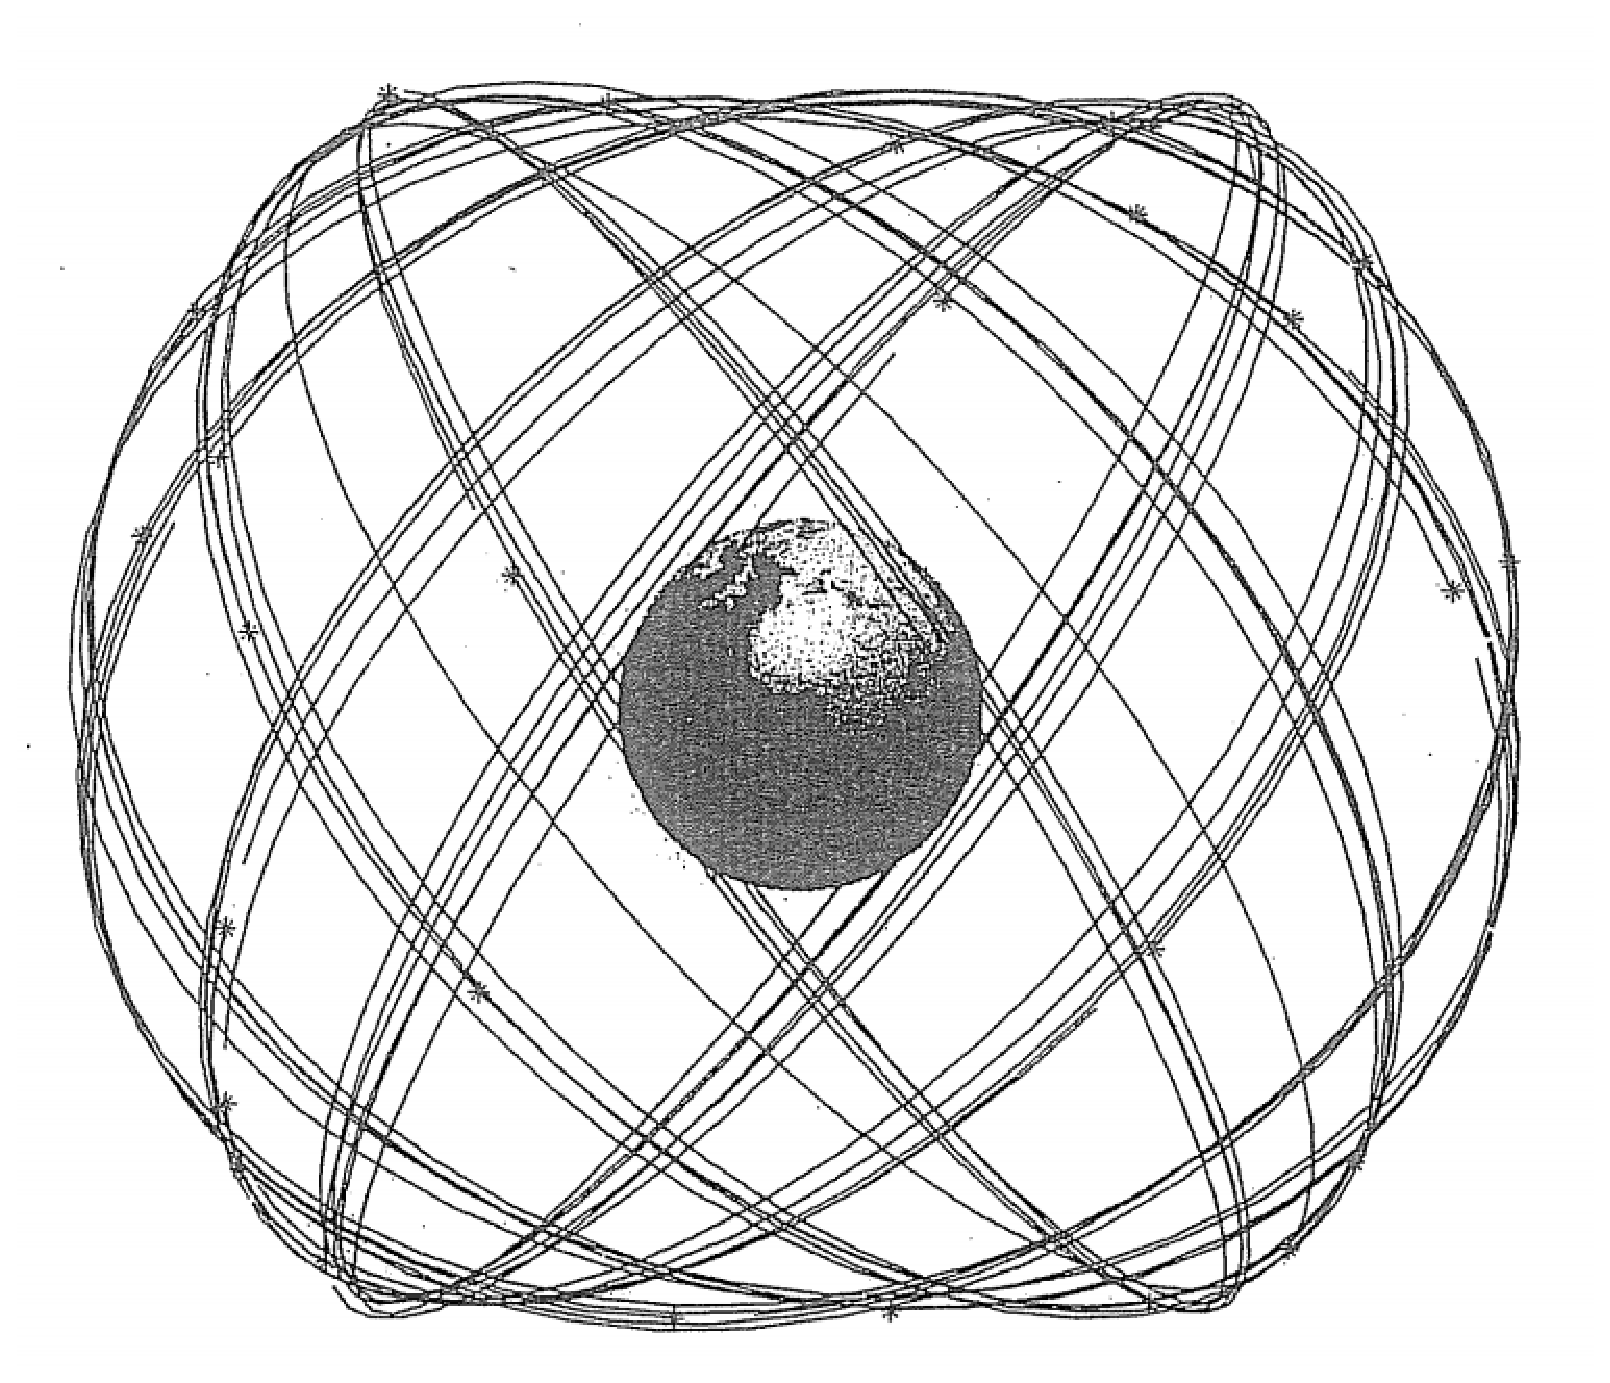
\includegraphics[width=0.4\linewidth]{TeX_files/Part03/chapter09/image/9-1}
	\caption{卫星轨道惯性坐标系——轨道穿过赤道和格林威治子午线(0°纬度、经度0°)。GPS卫星星座有6个轨道面每个上面有4个卫星。绕轨道/天15分钟完成,生产小偏移在每个轨道。}
	\label{fig:9-1}
\end{figure}
\begin{table}\label{tab:9.1}
	\caption{EASY Suites的项目列表}
	\small %设置表格字体大小
	\begin{tabularx}{\textwidth}{cXc}
		\hline  \rule[-2ex]{0pt}{5.5ex}   名称  & 					专题 						  & 页码\\ 
		\hline  \rule[-2ex]{0pt}{5.5ex}  easy1  & 时间转换:时间、UTC、GPS时间、GPS周和GPS秒  		& 第\pageref{subsec:easy1}页 \\ 
		\rule[-2ex]{0pt}{5.5ex}  easy2  & 开普勒法则,使用卫星星历计算卫星位置 			 & 第\pageref{subsec:easy2}页  \\ 
		\rule[-2ex]{0pt}{5.5ex}  easy3  & 使用伪距观测值计算接收机在ECEF系下的坐标 		 & 第\pageref{subsec:easy3}页  \\ 
		\rule[-2ex]{0pt}{5.5ex}  easy4  & 使用伪距单独计算基线					   	    & 第\pageref{subsec:easy4}页  \\ 
		\rule[-2ex]{0pt}{5.5ex}  easy5  & 使用伪距和载波计算基线,观测值使用最小二乘求解 	& 第\pageref{subsec:easy5}页\\ 
		\rule[-2ex]{0pt}{5.5ex}  easy6  & 和上面相同,但是现在用卡尔曼滤波估算基线	  	   & 第\pageref{subsec:easy6}页  \\ 
		\rule[-2ex]{0pt}{5.5ex}  easy6e & 和例5相同,但是引入带权重的观测值 			   & 第\pageref{subsec:easy6e}页 \\
		\rule[-2ex]{0pt}{5.5ex}  easy7  & 估算接收机时钟偏移量 							& 第\pageref{subsec:easy7}页\\ 
		\rule[-2ex]{0pt}{5.5ex}  easy8  & 检查周跳和接收机时钟重置 						  & 第\pageref{subsec:easy8}页   \\ 
		\rule[-2ex]{0pt}{5.5ex}  easy9  & 各种坐标下的给定基线 							& 第\pageref{subsec:easy9}页   \\ 
		\rule[-2ex]{0pt}{5.5ex}  easy10 & 估计电离层延迟对个别卫星的影响			 		& 第\pageref{subsec:easy10}页   \\ 
		\rule[-2ex]{0pt}{5.5ex}  easy11 & 卫星轨道的立体天球图和在当地局部范围的实时预报图 & 第\pageref{subsec:easy11}页   \\ 
		\rule[-2ex]{0pt}{5.5ex}  easy12 & 通过解释一个小的数值的例子来描述LAMBDA模型的细节 & 第\pageref{subsec:easy12}页   \\ 
		\rule[-2ex]{0pt}{5.5ex}  easy13 & 接收机自主完备性监测、水平防护和竖直防护等级 & 第\pageref{subsec:easy13}页   \\ 
		\rule[-2ex]{0pt}{5.5ex}  easy14 & 星基增强系统的样例,校正位置及其在斯坦福图中的呈现 & 第\pageref{subsec:easy14}页   \\ 
		\rule[-2ex]{0pt}{5.5ex}  easy15 & 对伪距单点定位、伪距基线结算和伪距载波联合观测的精度比较 & 第\pageref{subsec:easy15}页   \\ 
		\rule[-2ex]{0pt}{5.5ex}  easy16 & 筛选单向观测进行误差分析 							& 第\pageref{subsec:easy16}页   \\ 
		\rule[-2ex]{0pt}{5.5ex}  easy17 & 卫星轨道在惯性地固坐标系、地心地固坐标系下的图像 & 第\pageref{subsec:easy17}页   \\ 
		\rule[-2ex]{0pt}{5.5ex}  easy18 & 在基站计算不同的改正							 & 第\pageref{subsec:easy18}页   \\ 
		\hline 
	\end{tabularx} 
\end{table}	
原始观测数据是2001年9月4号位于奥尔堡(瑞士)的两台JPS Eurocard接收机收集的。最终生成的Rinex文件分别是site247j.01o、site24$\sim$1.01o、site247j.01n。对于其他需要长时间连续观测的特殊专题,它们所使用的文件被包含在kofi1.01o中。

上面所有提及文件的压缩包在网上都可以获取,网址是http://gps.aau.dk/~borre/esay/和http://gps.aau.dk/~borre/esay2/。
	\subsection[卫星轨道]{卫星轨道\\Orbits of the Satellites}
	卫星的轨道高度大约为3倍的地球半径。轨道接近于圆形,两个完整的轨道为一个恒星日。根据经验伪距观测值在卫星的高度角最小为$10^\circ$或大于$15^\circ$的范围时最可靠。图9.1显示了二维的早期24星的GPS星座图,在这6个轨道面上每一个都有四颗卫星。现在我们有31颗卫星。


	\label{subsec:easy17}\subsection[例子17]{例子17\\easy17}
	
	初学者对卫星轨道的样子实际上经常会有不同的想法。今天由30颗卫星组成的星座在6个不同的轨道面上,轨道面和赤道的夹角为$55^\circ$和之前的轨道面相比这个旋转了$60^\circ$.图\ref{fig:9-1}显示的情况看起来好像距离很远,因此我们叫做惯性参考框架。
	\begin{figure}
	\centering
	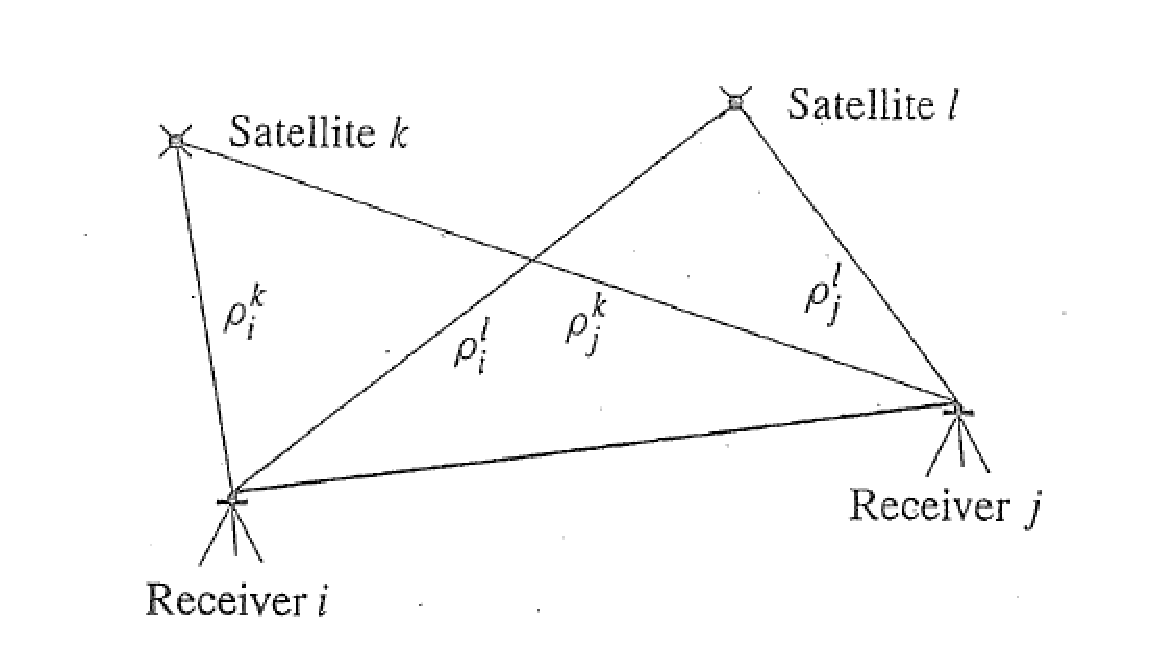
\includegraphics[width=0.4\linewidth]{TeX_files/Part03/chapter09/image/9-2}
	\caption{在ECEF框架下的卫星轨道}
	\label{fig:9-2}
	\end{figure}

	然而当这幅图像在旋转的地球平面上就显得不太清楚了。轨道到底是什么样的呢?非常奇怪。图\ref{fig:9-2}描述了这一情况。现在我们使用的是叫做地心地固坐标系(ECEF)。ECEF坐标系和旋转的地球具有固定的联系。那就是,给定一个点在一个坐标框架下的平面内是固定,除了那些可以移动的壳?(不懂)
	\begin{figure}
	\centering
	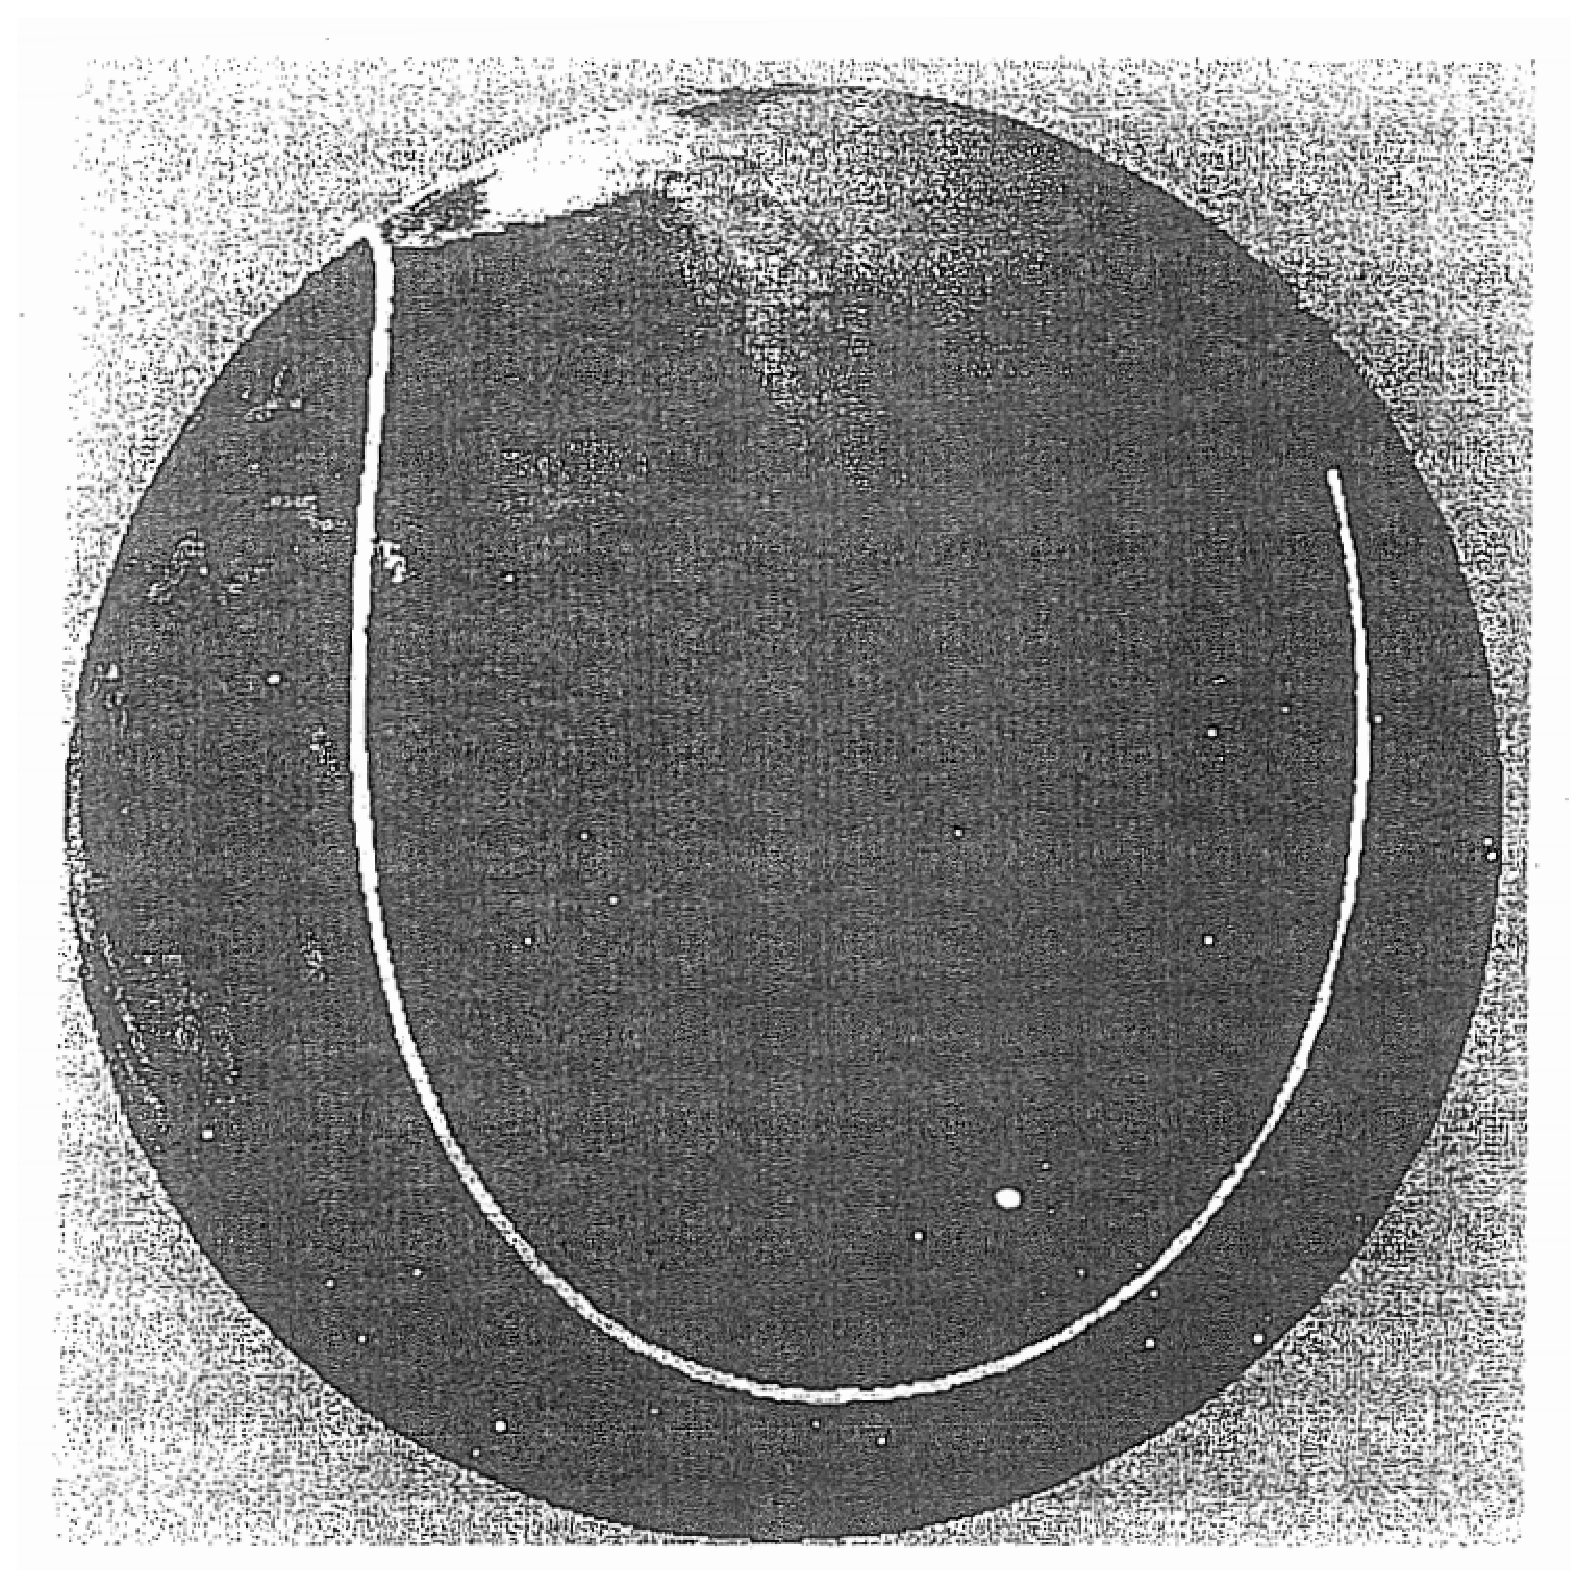
\includegraphics[width=0.4\linewidth]{TeX_files/Part03/chapter09/image/9-3}
	\caption{子卫星点选择的卫星。子卫星的曲线是由点的任意一个轨道的一部分。曲线之间的交点是地球表面和地球中心连线到卫星。}
	\label{fig:9-3}
	\end{figure}

	最后图9.3显示的曲线是子卫星在轨道上任意点的图像。这个曲线和地球中心到卫星的连线所在平面相交。子卫星的轨道在赤道两侧是对称的。这限制了向北和向南的对于轨道和赤道的夹角。
	\newpage